\newif\ifvimbug
\vimbugfalse

\ifvimbug
\begin{document}
\fi

\exercise{Expectation-Maximization}

In this exercise your task is to control a 2-DoF planar robot to throw a ball at a specific target. You will use an episodic setup, where you first specify the parameters of the policy, evaluate them on the simulated system, and obtain a reward. The robot will be controlled with the Dynamic Motor Primitives (DMPs).
The goal state of the DMPs is pre-specified and the weights of the DMP
$\theta_i, i = 1 \ldots 10$ are the open parameters of the control policy. Each DoF of the robot is controlled with a DMP with five basis functions. The ball is mounted at the end-effector of the robot and gets automatically released at time step $t_{\textrm{rel}}$.
We define a stochastic distribution $\pi(\vec{\theta}|\vec{\omega}) =
\mathcal{N}(\vec{\theta}|\vec{\mu},\boldsymbol{\Sigma})$, with $\vec{\omega} = \{\vec{\mu},\boldsymbol{\Sigma} \}$. \\
Your task it to update the parameters $\vec{\omega}$ of the policy using EM to maximize the expected return. In this exercises we will not
modify the low-level control policy (the DMPs) of the robot. 

A template for the simulation of the 2-DoF planar robot and plotting functions can be found at the course website. For the programming exercises, attach snippets of your code.

\begin{questions}


\begin{question}{Analytical Derivation}{5}

Using the weighted ML estimate,
\begin{equation}
    \vec{\omega}_{k+1} = \underset{\vec \omega}{\arg\max} \{ \sum_i w^{[i]} \log \pi(\vec{\theta}^{[i]};\vec{\omega})\},
\end{equation}
derive analytically the update rule for our policy $\pi(\vec{\theta}|\vec{\omega})$ for the mean $\vec{\mu}$. Show your derivations.

\begin{answer}
\begin{equation}
	\frac{\partial \vec{w}_{k+1}}{\partial \vec{\mu}} = 0
\end{equation}

\begin{equation}
 \pi (\theta^{[i]}; w) = N(\vec{\theta}|\vec{\mu},\boldsymbol{\Sigma}) = \frac{1}{\sqrt{(2\pi)^k |\boldsymbol{\Sigma}|}} exp(-\frac{1}{2} (\vec{\mu}-\vec{\theta})^T\boldsymbol{\Sigma}^{-1}(\vec{\mu}-\vec{\theta}))
\end{equation}

\begin{equation}
log(\pi (\theta^{[i]}; w)) = -log(\sqrt{(2\pi)^k|\boldsymbol{\Sigma}| })-\frac{1}{2} (\vec{\mu}-\vec{\theta})^T\boldsymbol{\Sigma}^{-1}(\vec{\mu}-\vec{\theta})
\end{equation}

\begin{equation}
\frac{\partial}{\partial \vec{\mu}}log(\pi (\theta^{[i]}; w)) = -\frac{1}{2}(2 \boldsymbol{\Sigma}^{-1} \vec{\mu} -2\boldsymbol{\Sigma}^{-1} \vec{\theta})
\end{equation}


\begin{equation}
\frac{\partial \vec{w}_{k+1}}{\partial \vec{\mu}} = 0 \rightarrow \sum_i w^{[i]} \boldsymbol{\Sigma}^{-1} {\mu}_i = \sum_i w^{[i]} \boldsymbol{\Sigma}^{-1} \theta_i \rightarrow \mu_i = \frac {\sum_i w^{[i]} \theta_i}{\sum_i w^{[i]}}
\end{equation}

\end{answer}

\end{question}

%----------------------------------------------


\begin{question}{Programming Exercise}{15}
Implement the EM algorithm using the provided framework. Your goal is to throw the ball at $\vec x = [2,1]m$ at time $t=100$. Use the weighted Maximum Likelihood (ML) solutions for updating the parameters of the policy. For the mean, use the equation derived at the previous exercise. For the covariance, the update rule is 
\begin{equation}
	\vec \Sigma_\mathrm{new} = \frac{\sum_i w^{[i]} (\vec{\theta}^{[i]}-\vec{\mu}_{\mathrm{new}})     (\vec{\theta}^{[i]}-\vec{\mu}_{\mathrm{new}})^T}{\sum_i w^{[i]}}.
\end{equation}
To calculate the weights $\vec{w}_i$ for each sample, transform the returned rewards by 
\begin{equation}
	\vec w^{[i]} = \exp ( ( \vec{R}^{[i]}(\vec{\theta}) - \max(\vec{R}) ) \beta )
\end{equation}
and normalize them, where the vector $\vec R\in \mathbb{R}^{N \times 1}$ is constructed from the rewards of the $N$ samples. The
parameter $\beta$ is set to
\begin{equation}
	\beta = \frac{\lambda}{ \max(\vec{R}) - \min(\vec{R}) },
\end{equation}
where $\lambda = 7$. Start with the initial policy 
\begin{equation}
	\pi(\vec{\theta}|\vec{\omega}) = \mathcal{N}(\vec{\theta}|\vec{0}, 10^6  \vec{I})
\end{equation}
and calculate the average reward at each iteration. Iterate until convergence or for a maximum number of 100 iterations.
We assume that convergence is achieved when the average return does not change much at every iteration, i.e., 
$$ | <\vec{R}_{i-1}> - <\vec{R}_\textrm{i}> | < 10^{-3}, $$
where $<\cdot>$ denotes the average operator.
At each iteration use 
$ N = 25 $ samples. In order to avoid getting stuck to a local optimum, we force the algorithm to explore a bit more by adding a regularization factor to the covariance of the policy,
\begin{equation}
    \vec{\Sigma}_\mathrm{new}^\mathrm{'} = \vec{\Sigma}_\mathrm{new} + \vec{I}.
\end{equation}
What is the average return of the final policy? 
Use \texttt{animate\_fig} from \texttt{Pend2dBallThrowDMP.py} to show how the final policy of the robot looks like (attach all five screenshots).

\begin{answer}
Average Return of the final policy: -38.89
\begin{center}
	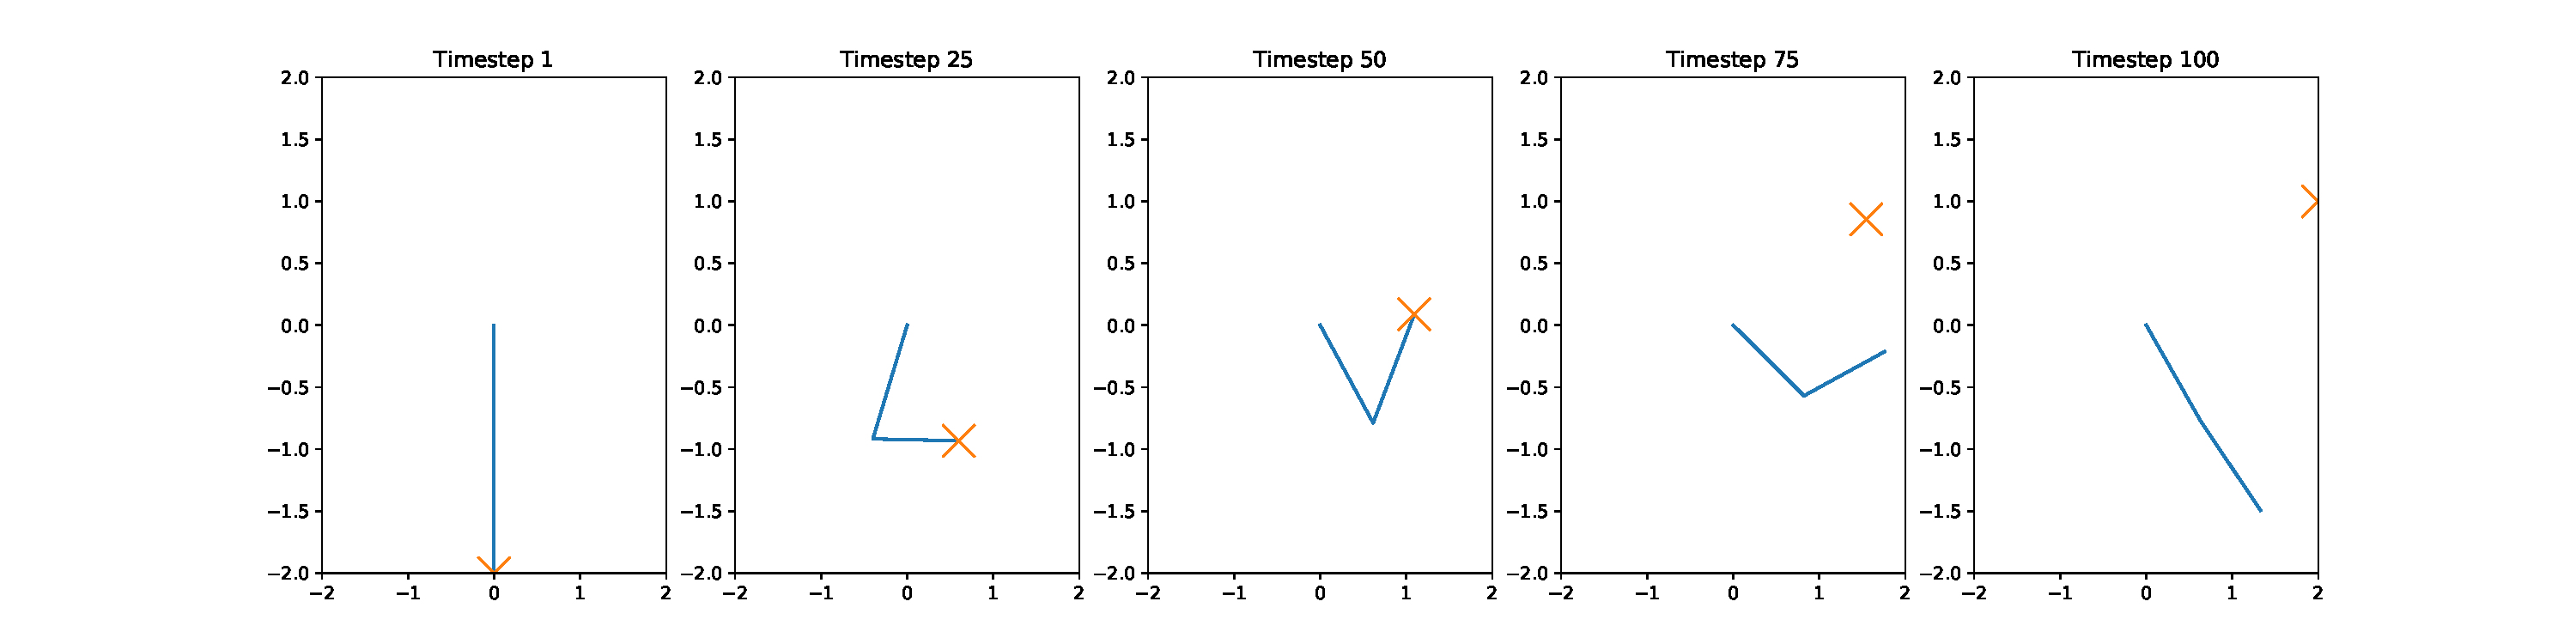
\includegraphics[width=1\textwidth]{img/EM-b.pdf}
	\captionof{figure}{Policy of the Robot's arm (blue) and the Ball's position (yellow cross)}
\end{center}
\end{answer}

\end{question}


%----------------------------------------------

\begin{question}{Tuning The Temperature}{5}
Repeat the learning 10 times and plot the mean of the average return of all runs with $95\%$ confidence for temperatures $\lambda = 25$, $\lambda = 7$ and $\lambda = 3$. How does the value of $\lambda$ affect the convergence of the algorithm in theory and what do you observe in the results? 
Use the logarithmic scale for your plot.

\begin{answer}
In the results we observe, that for $\lambda=25$ the average return converges faster than for smaller lambdas. Moreover it should be noted that for $\lambda=7$ we have the smallest average return at episode=100.\\

In Theory: With the temperature $\lambda$ one can select how the maximum of the weights is selected:
\begin{equation}
	\lim_{\lambda \rightarrow \infty} w^{[i]}: \text{weights are selected deteministically}
\end{equation}

\begin{equation}
\lim_{\lambda \rightarrow 0} w^{[i]}: \text{weights are selected stochastically}
\end{equation}

In the plots we can prove that for small lambdas the convergence is slower because the weights are selected stochastically. However the mean of the average reward for the last episode should be the smallest if the lambda is very small. This theoretical fact differs from the plot above.
\end{answer}

\begin{center}
	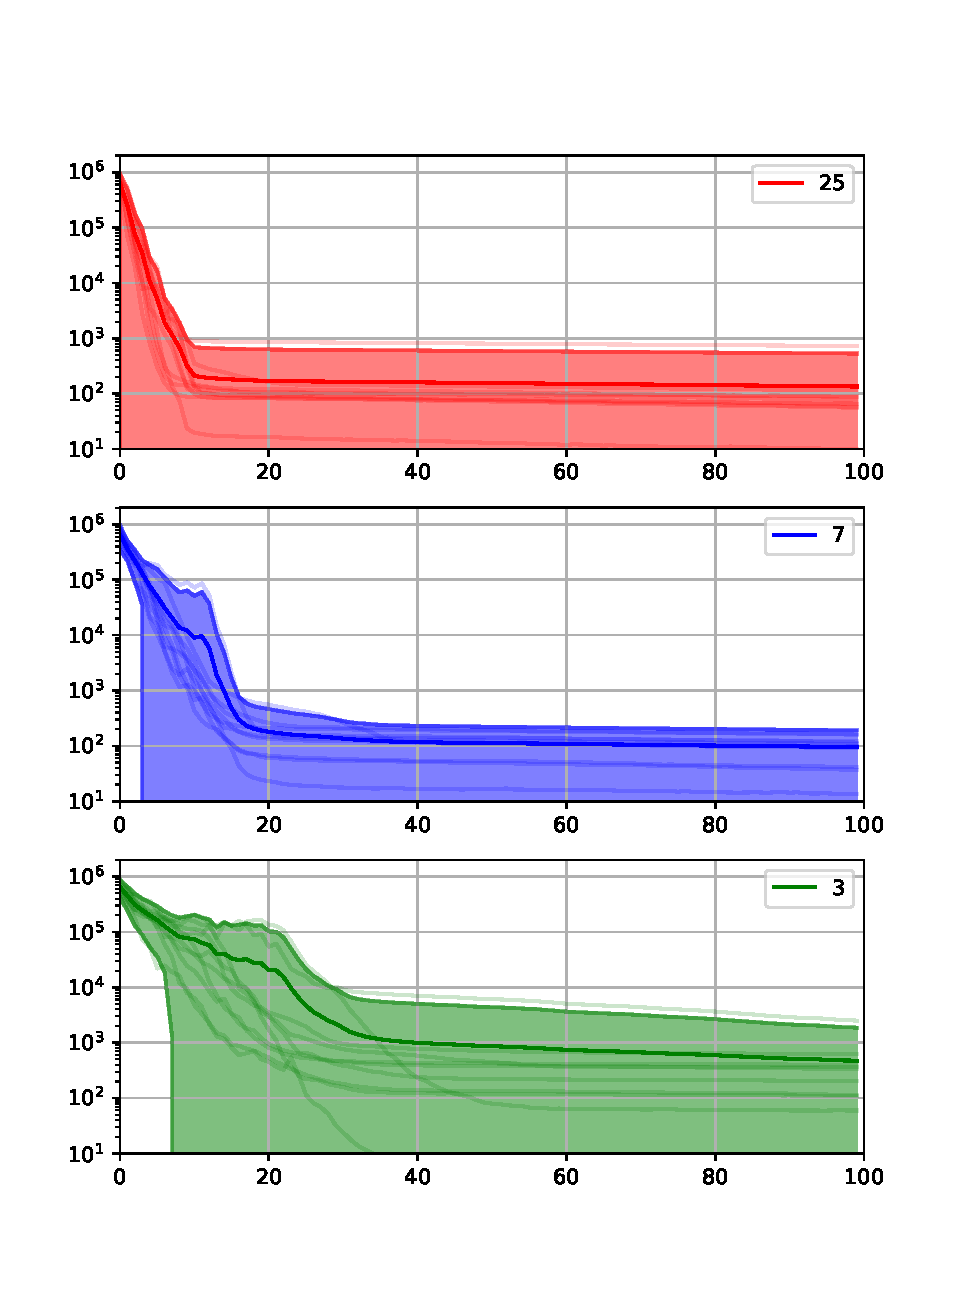
\includegraphics[width=0.5\textwidth]{img/EM-c.pdf}
	\captionof{figure}{The average return of different $\lambda$ over the episodes of the EM-Algorithm. }
\end{center}

\end{question}

%----------------------------------------------

\begin{question}[bonus]{Optimal Temperature}{5}
The problem of choosing $\lambda$ falls under a more general RL problem. Which one?
Which algorithm would allow you to automatically select the optimal $\lambda$? Explain it with your words.
Does it still have hyperparameters to be set?

\begin{answer}
RL problem: Policy Search Methods using Policy Gradients finding the right weights scaling factor. 
\\
 Algorithm that selects automatically the right lambda: Reward Weighted Regression.

The Reward Weighted Regression\\ is an algorithm that generalizes the EM algorithm. This algorithm reduces the problem of learning with immediate rewards to a reward-weighted regression problem with an adaptive, integrated reward transformation for faster convergence.  The resulting algorithm is efficient, learns smoothly without
dangerous jumps in solution space, and works well in applications of complex high degreeof-freedom robots.

Hyperparameters:\\
A transformed Hyperparameter still has to be set in RWR. However this parameter is automatically updated. With this parameter the convergence speed can be selected.
\end{answer}


\end{question}


\end{questions}

